\section{Causas raíz}
Como se detalla en el diagrama de Ishikawa (Figura \ref{fig:ishikawa}), la interrupción no fue producto de un ciberataque (síntoma), sino de un fallo de configuración interno. La causa raíz técnica se originó durante la transición a la nueva arquitectura Multi-Colo PoP (MCP), cuando un error operativo al reordenar los términos de las políticas de enrutamiento BGP provocó el retiro involuntario de prefijos de red críticos en los enrutadores perimetrales \cite{cloudflare2022}.

\begin{figure}[htbp]
    \centering
    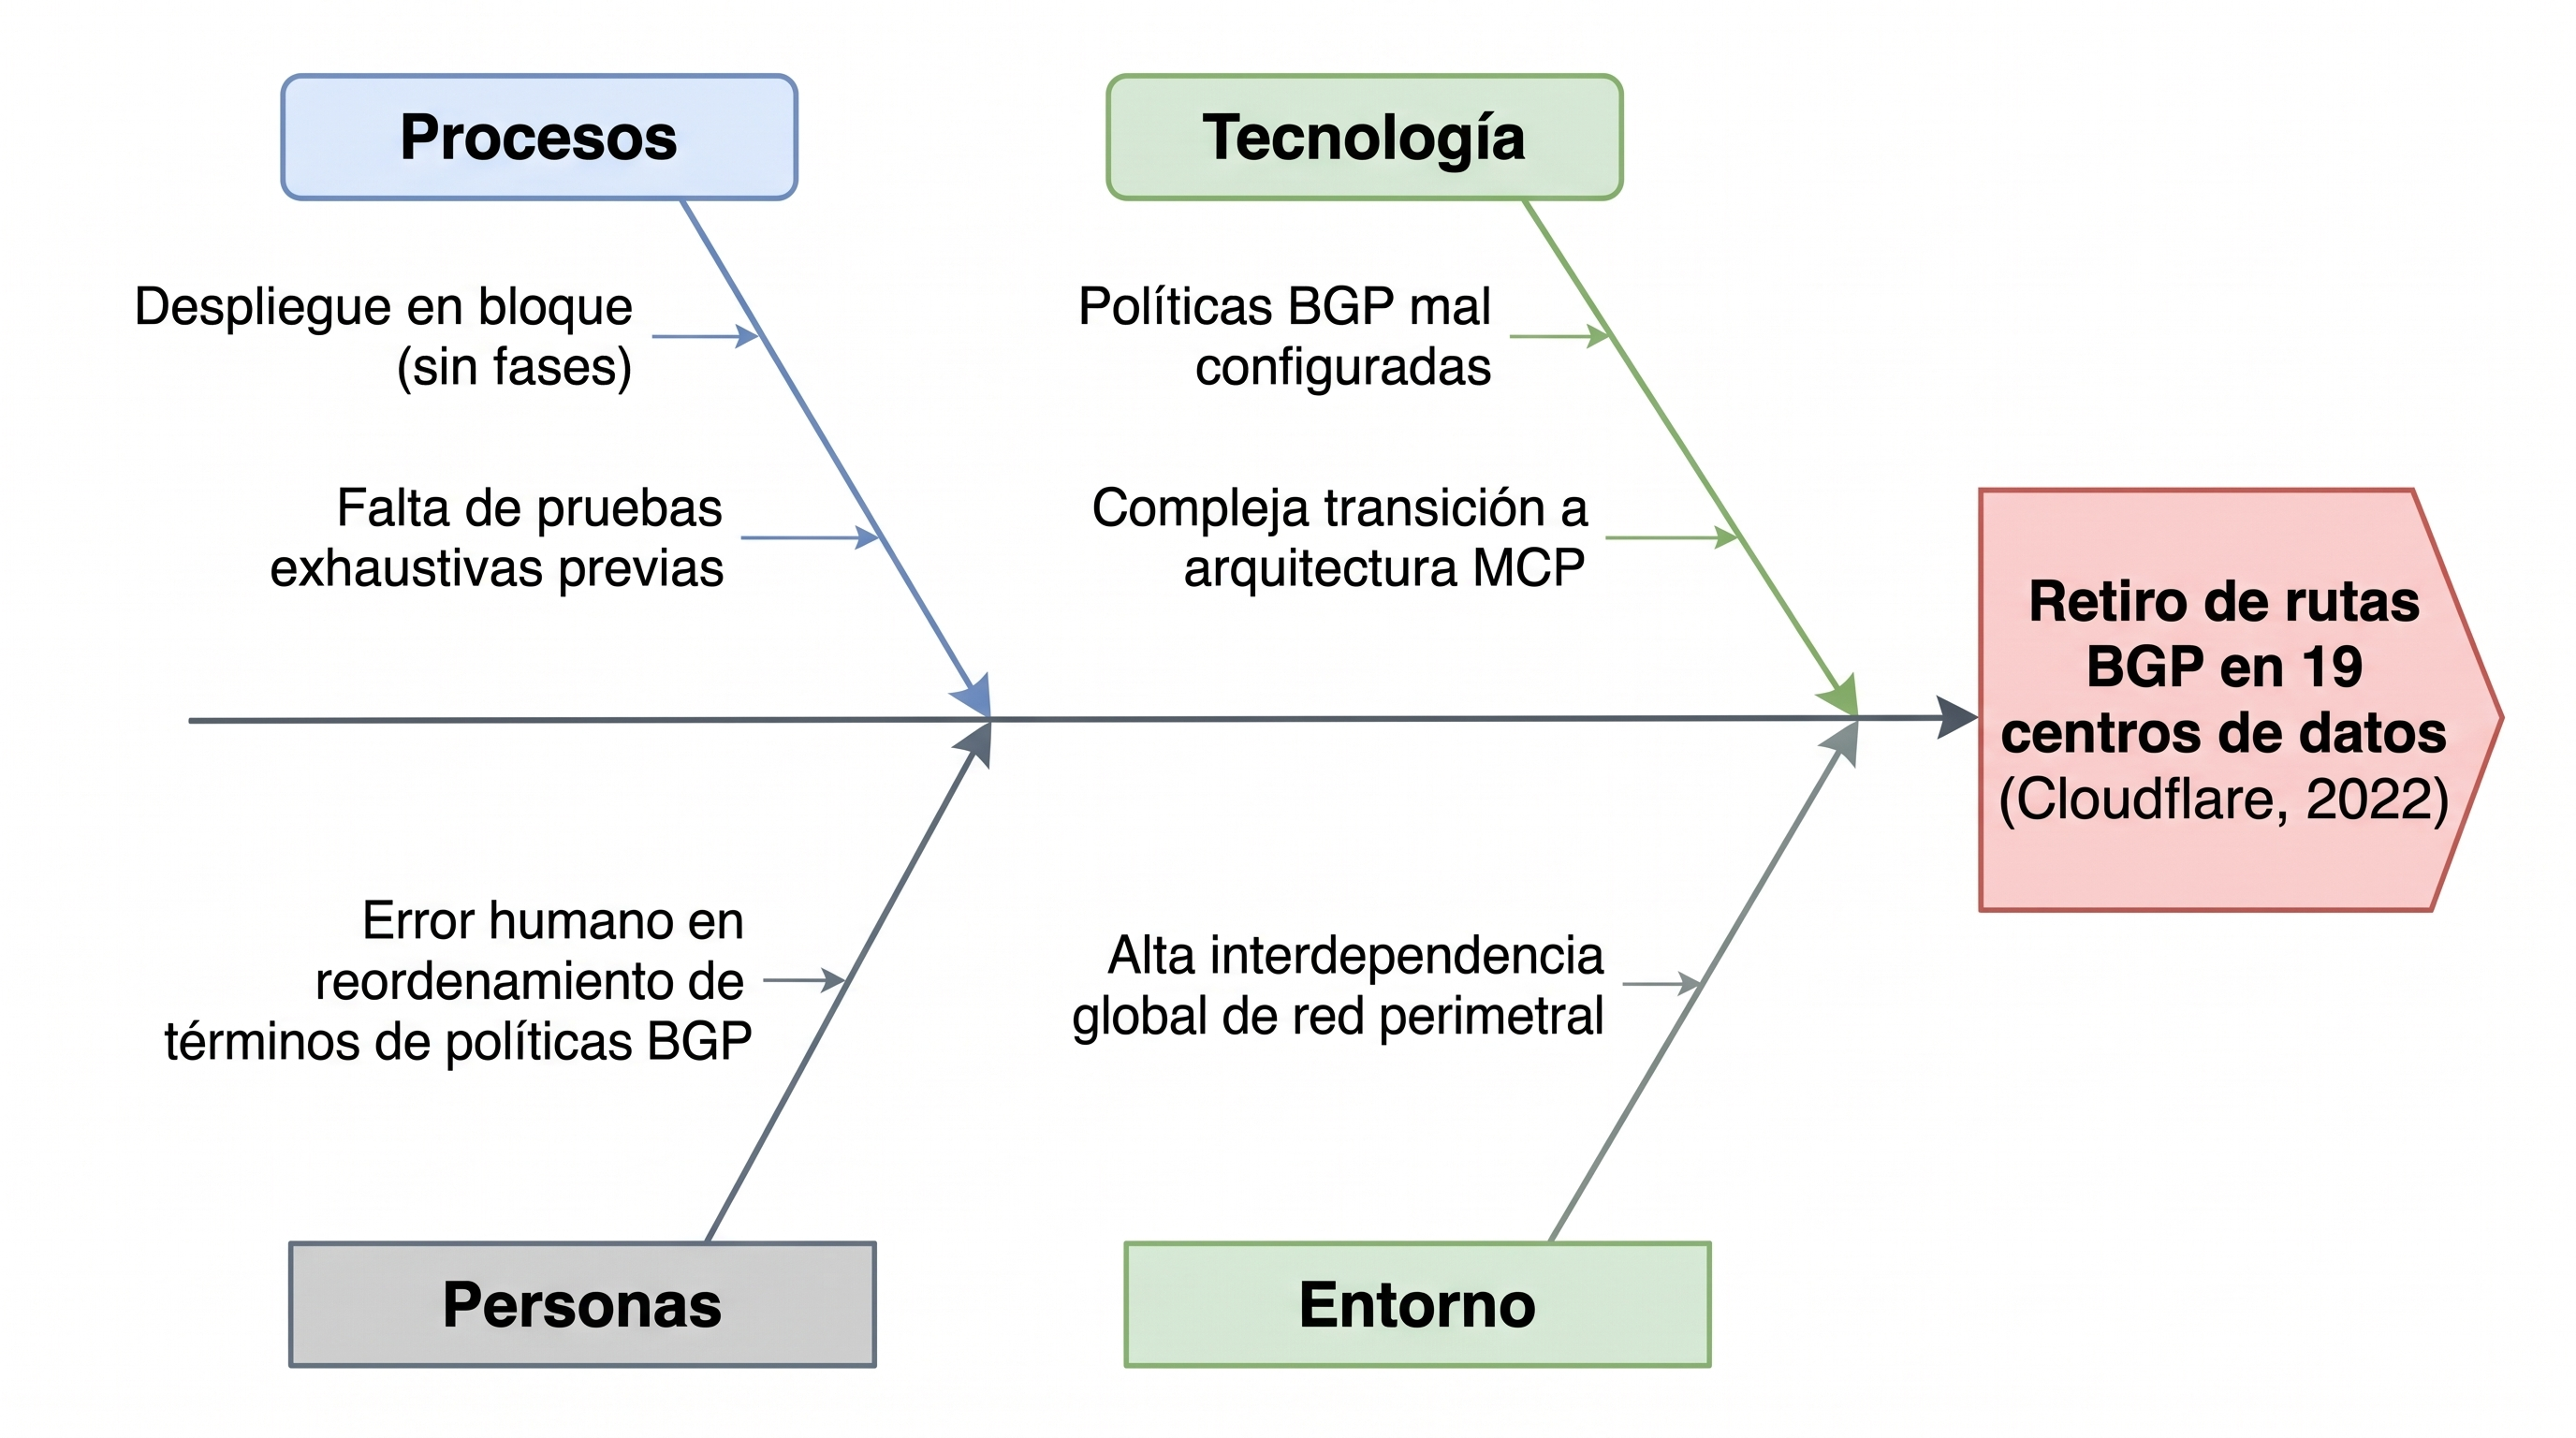
\includegraphics[width=\textwidth]{diagramas/ishikawa-cloudflare-2022}
    \caption{Diagrama de Ishikawa elaborado por el equipo con las causas del incidente.}
    \label{fig:ishikawa}
\end{figure}
